\subsection{Siemens case}
Siemens Wind Power is among the leading windmill manufacturers in the world. 
Siemens builds wind farms of different sizes ranging form single mills to well above one hundred windmills \cite{simensOffShoreProjects, simensOnShoreProjects}.

In the current setup (see \cref{fig:currentSiemensSetup}) the Park Monitor is a central component and a SPOF (single point of failure).
The system is running on windows with a MSSQL database in the Park Monitor and MySQL on the windmills them self.
The windmills, Park Monitor and Park Regulator is connected with a gigabit network, witch currently has plenty of extra capacity.
The system handles more than 50 control points and 200 measurement points, and samples these every 50 ms.
The Park regulator is associated with the transformer station and regulated the power production when needed.
This component currently has a less than optimal work flow see \cref{fig:dataComputationSequence}.

Siemens has a need for their system to scale better and provide increased redundancy to avoid these SPOF's.
Siemens has a vision of removing the Park Monitor component and make it into a distributed system, distributed among the windmills. % (see \cref{fig:futureSiemensSetup}).
Also Siemens would like to look for ways to optimise the calculations done by the Park Regulator.

\begin{figure}
	\centering
	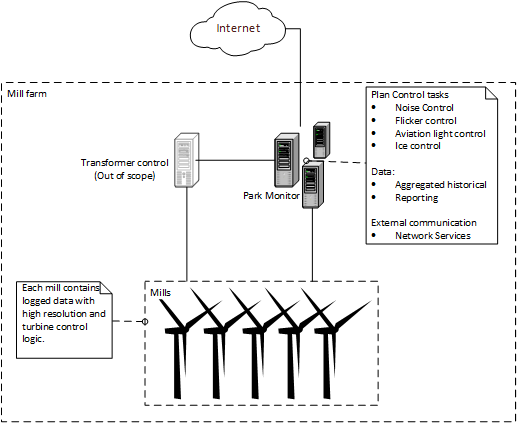
\includegraphics[width=0.7\textwidth,natwidth=610,natheight=642]{SystemOverviews.png} 
	\captionsetup{format=plain,font=footnotesize,labelfont={bf,red},labelsep=quad,singlelinecheck=no}
	\caption[Illustrates the current Siemens windmill farm setup]{
		\label{fig:currentSiemensSetup} 
		\footnotesize{%
			This figure illustrates the current Siemens windmill farm setup.
		}
	}
\end{figure}

%\begin{figure}
%	\centering
%	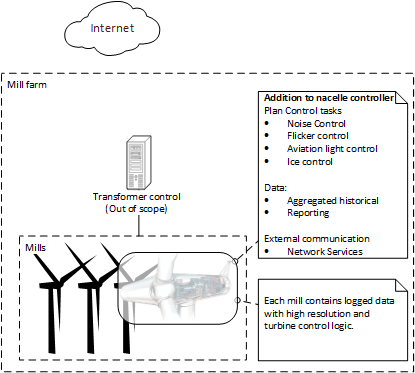
\includegraphics[width=0.7\textwidth,natwidth=610,natheight=642]{SystemOverviewsFuture.png} 
%	\captionsetup{format=plain,font=footnotesize,labelfont={bf,red},labelsep=quad,singlelinecheck=no}
%	\caption[Illustrates the future Siemens windmill farm setup]{
%		\label{fig:futureSiemensSetup} 
%		\footnotesize{%
%			This figure illustrates the future Siemens windmill farm setup.
%		}
%	}
%\end{figure}

\begin{figure}
	\centering
	\begin{sequencediagram} %Created using pgf-umlsd
		\newthread{reg}{:Park Regulartor}
		\newinst[2]{mill}{:Mill}
	
		\begin{sdblock}{each mill}{}
			\mess[1]{reg}{getCurrentStatus}{mill}
			\mess[1]{mill}{status}{reg}	
		\end{sdblock}
		
		\begin{call}{reg}{calculateAllSetpoints()}{reg}{}
		\end{call}
	
		\begin{sdblock}{each mill}{}
			\mess[1]{reg}{setNewSetpoint}{mill}
		\end{sdblock}
					
	\end{sequencediagram}

	\captionsetup{format=plain,font=footnotesize,labelfont={bf,red},labelsep=quad,singlelinecheck=no}
	\caption[Regulator calculation sequence]{
		\label{fig:dataComputationSequence} 
		\footnotesize{%
			Regulator calculation sequence.
		}
	}
\end{figure}














